\chapter{Implementation}\label{C:impl}

\section{Front End}  %this needs a better title, badly.

web application, written using javascript, css and html5.

Figure \ref{overview} shows an overview of the Honeynet dataset. In a column to the left, we have some controls for the visualisation. To the right, taking up the majority of space is a timeline visualisation of logged data.  
Basic interaction is carried out with the mouse primarily. Filtering and datetime controls are located in a panel to the left of the screen. The remainder of screen space is taken up by the timelines. 
Each of the four stacked timelines covers a fixed period, with each line starting when the line above ends. The times displayed in the control panel show the start time of the first timeline, and end time of the last timeline.
Doubleclicking on any timebin triggers a zoom action, replacing the contents of all timelines with a more detailed view of the chosen bin. 
No functionality was included to go back up a zoom level, as the application does not currently know what times were in view before the current. Instead, the application has been integrated with the browser history. The browser back and foward buttons serve to step through states, including zoom levels. 

Zooming can be performed until either there is only one event in the chosen bin, or each bin covers 1 second. The one second limit is a practical consideration of the structure of SSHD logs. These logs have a time resolution of 1 second, ie:  all events occuring between 10:59:59.000 and 11:00:00.999 are logged at 10:59:59. Where there is only one event to display, mousing over the bin will show the raw log line in a popup. This was implemented to reduce the number of zoom actions required to see details in low activity time blocks. 

This approach provides an arbitrarily large number of zoom levels, with more detailed statistical summaries of each block presented by mouseover<insert link to screenshot>. This was implemented to support information hiding requirements. 

Filtering functions are currently somewhat limited, with options to show only data for a given username, IP addres, and toggle the display of each class of event. These filters can be freely combined. IP and username filters support wildcards, \_ matches a single character, \% matches 1 or more characters. 

This is a purely visual change, with no change in data, this can be seen as mousing over the bins shows the same summary information. These filters were implemented without altering the selected data to support exploration of potential attacks. ie: when looking for a brute force attack against root, I would hide failed attacks, as there are vastly fewer successful root logins, Then use the mouseover breakdown to check which (if any) bins had a suspiciously high failure rate. This would not be possible were the data to be filtered on the server side, as currently implemented the statistical summary would lose details.

  

(discuss why data is currently reloaded due to issues in history api.) 
<Explain basic interactions here, related back to functional and nonfunctional requirements.>
<explain why features were cut, here or design?>

Both date boxes are linked to datepicker tools, which allow for chosing a date from a calendar, and setting time through sliders. These values may be freely edited without reloading data. The Jump to dates button will trigger a reload of data. 
Binlength (Immediately below date controls) allows chosing the length of each timebin. the dropdown controls units (from seconds to years), while the textbox accepts a number of units.
<Complete detailed description>
\begin{figure}[h!]
\fbox{\parbox[b]{.99\linewidth}{
\centering 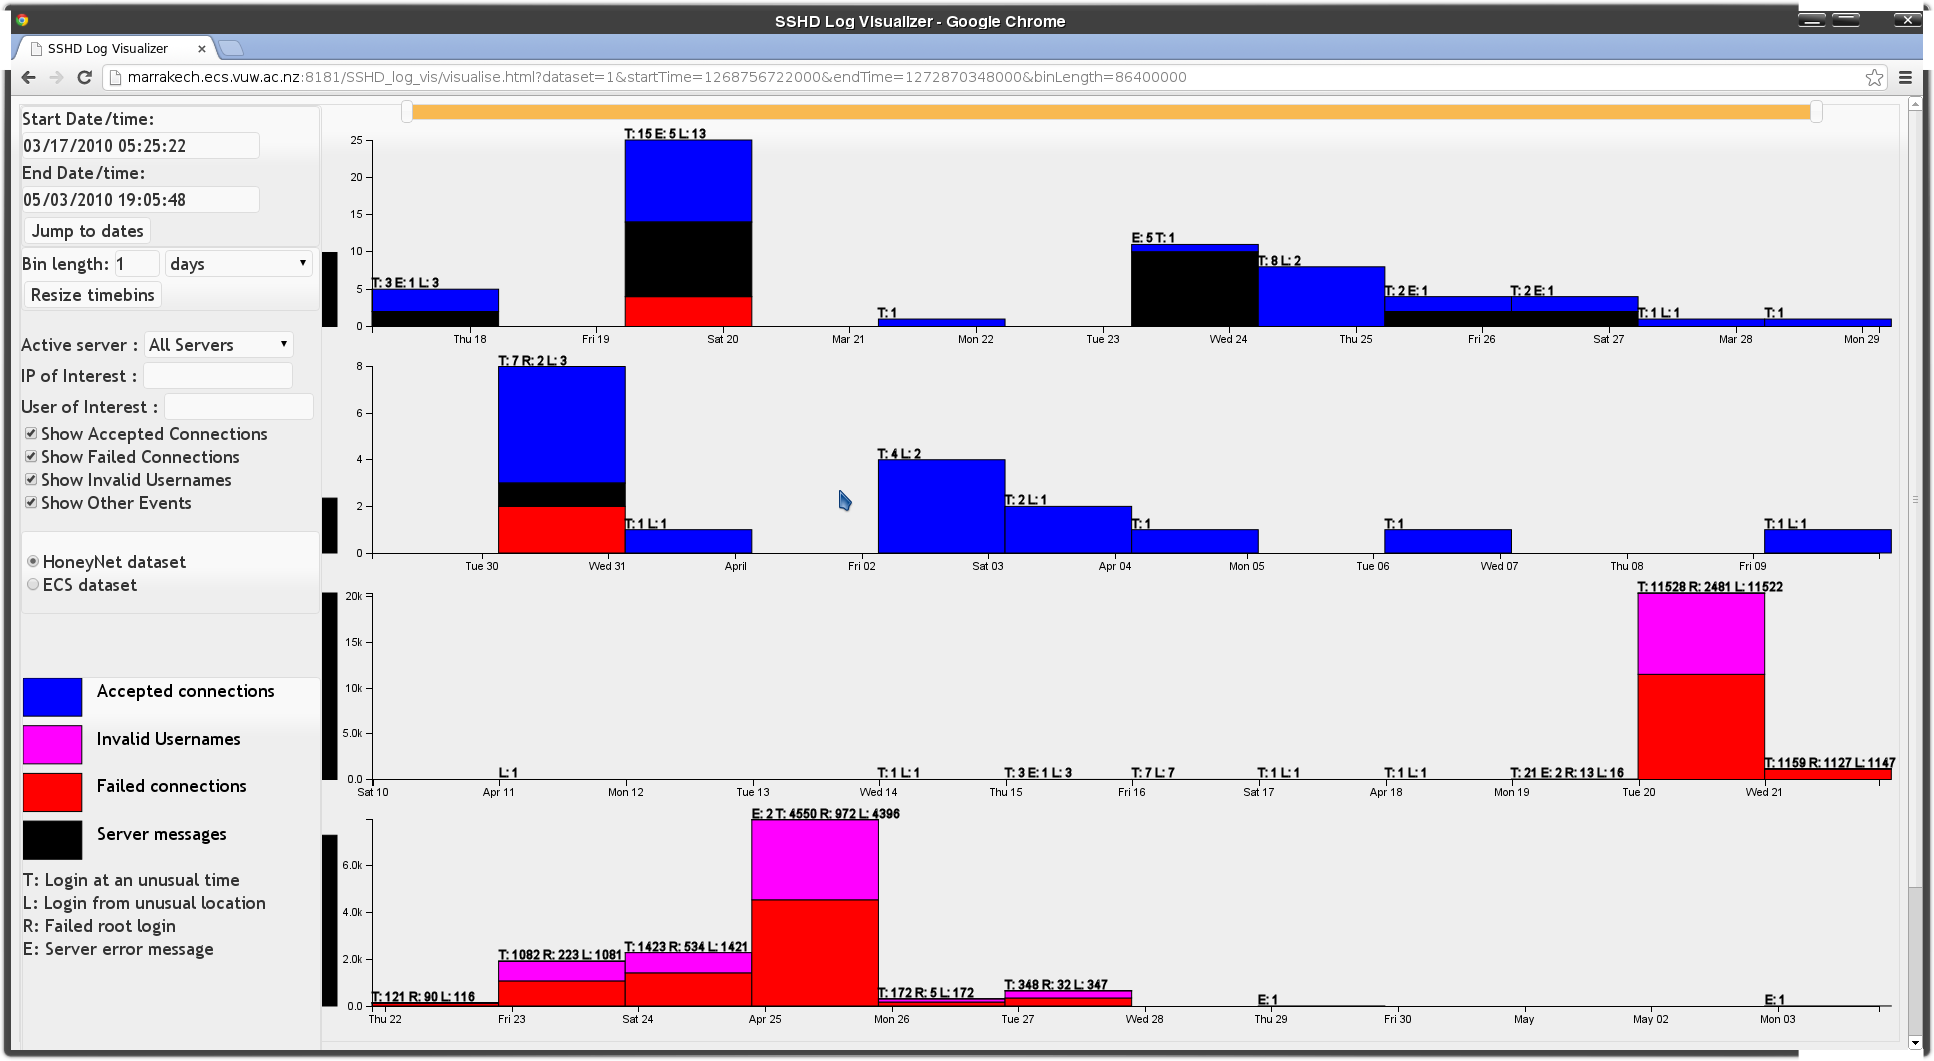
\includegraphics[scale=0.43,  angle=270]{screenshots/overview.png}
}}
\caption{\protect\label{overview}Tool showing overview of the honeynet dataset (\ref{data})}
\end{figure}


\section{Database}\label{imp_db}
Few issues were encountered with the MySql RDBMS used for the project. Two major issues arose, both causing severe performance problems for the parsing tool. One issue was related to index use for range queries, the other represented a limitation of the default java database connection system. 

GeoIp data presented a significant problem during the implementation phase of this project. I made use of the free GeoLite geoIp database, which is provided as a pair of CSV files. IP addresses in this database are represented as 32 bit unsigned integers, with a start and end column defining a range.

The extreme slowness of these queries caused unacceptable performance for the parser due to use of GeoIP information during location clustering. For batch loads potentially tens of thousands of queries would be made to the GeoIP table. Honeynet data consists of 35006 rows, of which 20469 rows resulted in GeoIp lookup. In the ECS dataset, 14885 of 75K rows resulted in GeoIp lookups. 

This design has some unfortunate implications for query efficiency, as there are approximately 2 million ranges<look up the exact number>. Range queries across two columns (constant between ColumnA and ColumnB) cannot use an index in most RDBMS systems. This results in very poor performance for queries.
Some simple optimizations are possible, assuming that ranges are non overlapping, and exhaustive. (ie: every address is in exactly 1 range)  With this assumption, a simple query selecting the first range where IP greater than or equal start, in increasing order by start will always select the matching range.

However it's uncertain if the ranges in the dataset are both exhaustive and non overlapping. Checking this property would take significant time and effort, and would need to be repeated  every time the dataset is updated (Monthly). Due to these issues, an alternative approach was sought, and found in the spatial extensions.

Using spatial extensions allows encoding the start and end numbers for IP ranges as a single shape, either line segment or square. Once so encoded, an IP can be range checked by creating a point from the address, and checking if the point is in any shapes. While this shape checking test is slower than a simple inequality test, the ability to use indexes improves performance significantly. Without spatial extensions, a range query may take many seconds, With spatial encoding this dropped to under 0.1 seconds.  

One drawback to spatial extensions for MySql is that they are not supported in the innoDB storage engine, which is the only MySql storage engine to offer transaction support. This is not a significant issue for GeoIP data, where all accesses are reads, exept for a complete table reload each time that the dataset is updated. This reload can be performed in under 5 minutes using batch loading tools available with MySql. As GeoIp databases are often updated only monthly or less frequently, this is an acceptable limitation. 

Shifting to spatially encoded ranges for GeoIp lookups was responsible for a significant improvement in loading times for batch loads. A further significant improvement was achieved by collecting groups of 1000 rows per insert transaction, as transaction overhead for the default JDBC autocommit behaviour was negatively impacting performance. 
 
\section{Parser}

The log parsing tool was implemented in two layers. A log reader, and database writer/analyser. 
The reader layer is responsible for reading any number of log files into a sorted list of events.
This list of events is then passed to the analyser/writer layer, which is responsible for checking connection attempts to see if the location and time are frequently used by the user and writing the analysed metadata to the datastore.

The writer layer is tightly coupled to both the database schema, and RDBM systems specifically as it makes extensive use of the JDBC api for communicating with RDBMS's.
Internal representation of log entries is somewhat coupled to the JDBC API, as each entry is responsible for binding its data to the prepared statements used by the writer.
This could be worked around with minimal changes so long as the new datasource implemented the same API.

Few significant issues were encountered in writing the parser. 
The majority of trouble encountered with the parser was in analysing connection attempts. checking weather a location  is one that is well known is extremely simple, though had significant performance issues discussed in \ref{imp_db}
Time clustering has proven to have ongoing issues, where overlaps in stored time ranges are not properly detected. This error arises where the number of successful login attempts is not correctly aggregated across all time sections which overlap the login attempt. This causes a significant number of false positives for unusual times. I believe that this bug is caused by an error in my SQL queries, though at time of writing this remains unresolved. 

\section{Server}

There were few issues with server implementation, as tomcat is well documented.
Some trouble initially setting up tomcat within university systems due to outdated instructions. 
Once this was resolved, servlet api is extremely well documented, with very good online tutorials. 
Biggest issues with server implementation occured in attempting to get responses to use compression to reduce the size of the resulting packets. Compression isn't really important, and all issues were caused by outdated tutorials. Once up to date documentation was found, enabling compression was trivial.
This can be done by server configuration files.
Remove this section? There really isn't a lot to say about server implementation. 


\subsection{Security Concerns}
The server is constrained to use a very old version of java, as the system was developed against an older version of tomcat. Exposing this version of the server to the internet is not advised, as it may contain unpached vulnerabilities. However, porting to a later version of tomcat should not involve any great difficulty.  Configuration files would need to be rebuilt, however there should not be any significant compatibility issues.

\section{Testing}
Automated testing of user interfaces remains problematic, with many tools suffering from severe fragility where UI layout is modified. In most testing libraries, mous interaction is recorded at test design, then played back artificially on execution, This causes severe fragility as if a control or button moves the recorded mouse movements will miss the button, causing test failures. Further research is needed to find a testing library suitable for testing, however the test automation tool created by Dojo appears useful \cite{dojo2013test}. - automated testing not used. heavy use of in browser dev tools and debugger. manual testing. 